\chapter{The Processor}
	\section{The Little Man Computer}
		The power of the computer does not arise from complexity, instead it comes from its ability to perform simple operations at an extremely high rate of knots. This means that actual design of a computer is also simple. We'll start our adventure in investigating the processor by looking at the Little Man Computer (LMC). Whilst it is not a physical computer it is a simplified model to allow us to understand the basics of computer architecture before moving on to looking at the more complex RM processor.
		
			\subsection{Physical Layout}
				\begin{figure}[t]
					\begin{center}
						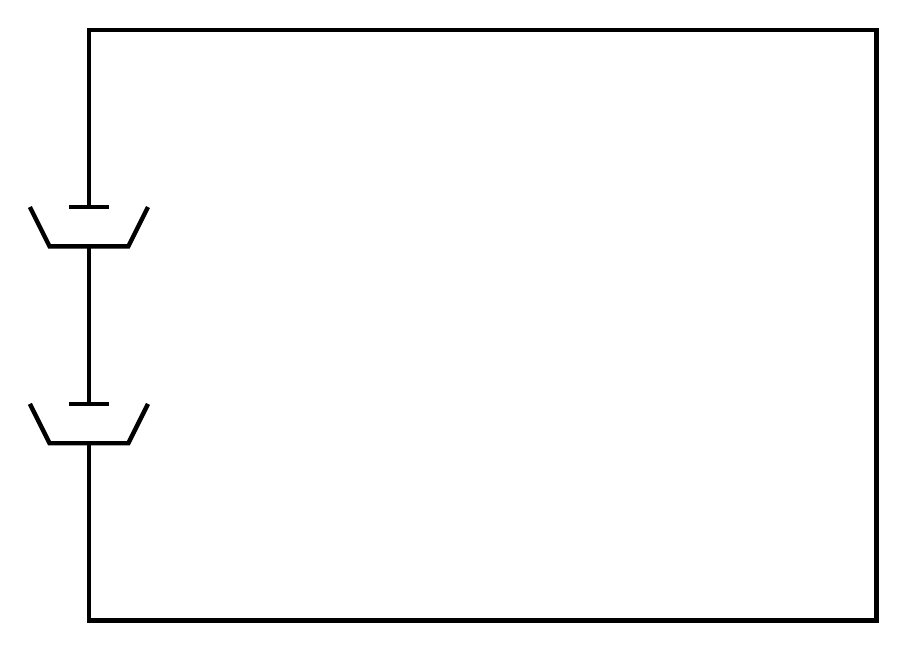
\begin{tikzpicture}[scale = 0.5]
							\draw[ultra thick] (0,4.5) -- (0,0) -- (20,0) -- (20,15) -- (0,15) -- (0,10.5);
							\draw [ultra thick] (0,9.5) -- (0,5.5);
							\draw [ultra thick] (-0.5,10.5) -- (0.5,10.5);
							\draw [ultra thick] (-1.5, 10.5) -- (-1,9.5) -- (1,9.5) -- (1.5, 10.5);
							
							\draw [ultra thick] (-0.5,5.5) -- (0.5,5.5);
							\draw [ultra thick] (-1.5, 5.5) -- (-1,4.5) -- (1,4.5) -- (1.5, 5.5);
							
						\end{tikzpicture}
					\end{center}
					\caption{\label{fig:LMCLayout} Layout of the Little Man Computer}
				\end{figure}
				We shall start by looking at the physical layout of the Little Man Computer, illustrated in Fig. \ref{fig:LMCLayout}. The LMC consists of a walled post-room, indicated by thick line. Inside this their are various items.
				\begin{itemize}
					\item \num{100} \textit{pigeon holes} - numbered with an address ranging from \numrange[minimum-integer-digits=2]{00}{99}. Each pigeon hole is designed to hold a single slip of paper, upon which is written a three digit decimal number. 
					\item  \textit{A Calculator} - the calculator is used to enter and temporarily hold numbers, and also to add or subtract. The display is three digits wide and there is no provision made for negative numbers
					\item A \textit{Hand Counter} - The type that you click to increment the count. There is a reset button located outside the post-room.
					\item The \textit{Little Man} - It is his role to perform certain tasks to be defined shortly.
					\item An \textit{in basket} and an \textit{out basket}. These allow a user to communicate with the Little Man by putting a three digit number into the in basket. Similarly the out box allows the Little Man to write a three digit number on a slip of paper and leave it in the out basket.
				\end{itemize} 
				
			\subsection{Instructions of the LMC}
				We would like the Little Man to do some useful work for us. For this purpose we have invented a small group of instructions that he can perform. Each instruction will consist of 3 digits. We use the first digit to tell the Little Man what instruction to perform, this is known as the opcode \index{Opcode}. The last two digits are known as the operand \index{operand} and tell the Little Man to get data to be used as part of the instruction. Figure \ref{fig:LMCoperand} shows the split of the instruction into its opcodes and operands. 
				
				\begin{figure}[h]
					\centering
					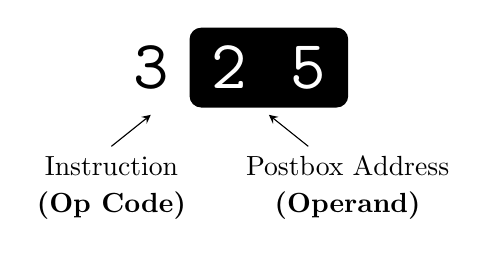
\begin{tikzpicture}
						\node at (0,0) {\Huge \texttt{3}};
						\draw[fill=black, rounded corners] (0.5,0.5) rectangle (2.5,-0.5);
						\node at (1,0) {\Huge \texttt{\textcolor{white}{2}}};
						\node at (2,0) {\Huge \texttt{\textcolor{white}{5}}};	
						\node at (2.5,-1.25) {Postbox Address};
						\node at (-0.5,-1.25) {Instruction};
						\node at (2.5,-1.75) {\textbf{(Operand)}};
						\node at (-0.5,-1.75) {\textbf{(Op Code)}};
						\draw [stealth-](1.5,-0.6) -- (2,-1);
						\draw [stealth-](0,-0.6) -- (-0.5,-1);	
					\end{tikzpicture}
					\caption{\label{fig:LMCoperand} The structure of an LMC command}
				\end{figure}
			
				Whilst the structure of the operand is relatively straight forward, \LMC{25} represents mailbox 25 for example, we need more information to decode the opcodes. The processor instruction set defines the instructions, and the machine codes that go with it. The are particular for each processor. \index{Instruction Set} \index{Processor Instruction Set|\see{Instruction Set}} \glossary{Processor Instruction Set}
				
				There are 11 different instructions that the Little Man has to decode. 
				\begin{description}
					\item[COFFEE BREAK (or HALT) - opcode 0] The little man takes a rest. He ignores the address portion of the instruction.
					\item[ADD - opcode 1] The Little Man walks over to the post-box specified in the instruction. He reads the three-digit number located in the mailbox and walks over to the calculator and \textit{adds it to the number already in the calculator}.
					\item[SUBTRACT - opcode 2] The Little Man walks over to the post-box specified in the instruction. He reads the three-digit number located in the mailbox and walks over to the calculator and \textit{subtracts it from the number already in the calculator}. \footnote{For the purposes of the model we'll assume that the calculator handles negative numbers correctly but the Little Man ignores any minus sign}.
					\item[STORE - opcode 3] The Little Man walks over to the calculator and reads the number there. He writes that number of a slip of paper and puts it in the post-box specified in the operand. The number in the calculator is unchanged specified in the instruction and the previous value is overwritten.
					\item[LOAD - opcode 5] Similar to the \LMC{ADD} instruction, the Little Man walks over to the post-box specified in the instruction. He reads the three-digit number located in the mailbox and walks over to the calculator and types it into the calculator. This leaves the original mailbox unchanged but the calculators previous value is overwritten.
					\item[BRANCH UNCONDITIONALLY (or JUMP) - opcode 6] This instruction tells the little man to walk over to the instruction counter and \textit{change} the counter to the location shown in the operand. 
					\item[BRANCH ON ZERO - opcode 7] The Little Man will walk over the calculator and observe the number stored there. If its current value is zero, he will walk over to the instruction location counter and modify its value to the address specified by the operand.
					\item[BRANCH ON POSITIVE - opcode 8] The Little Man will walk over the calculator and observe the number stored there. If its current value is \textit{positive}, he will walk over to the instruction location counter and modify its value to the address specified by the operand.
					\item[INPUT - opcode 901] The Little Man walks over to the basket and picks up the slip of paper in the basket. He then walks over to the calculator and punches it into the calculator. If there are multiple slips of paper the Little Man only takes the oldest.
					\item[OUTPUT - opcode 902] The Little Man walks over to the calculator and writes down the number that he sees there on a piece of paper. He walks over to the out basket and places the slip of paper there for the user.
					
					
				\end{description}
				
	\section{Processor Performance}
		\subsection{Number of Cores}
		
		\subsection{Cache Size}
		
		\subsection{Clock Speed}
		
		\subsection{Word Length}

	\section{Assembly Programming}
		
		\subsection{Registers}
			It is said that Assembly programming is programming by moving data. 
%		In order for our CPU to run efficiently we need quick access to the instructions operands. We could store all operands in the memory, which would be fine but due to the significant delay of introduced by having to send signals outside of the CPU to external memory we would have our processor sitting idle for large chunks of time. One solution to this is to use registers. These are storage devices that hold a word exactly like a memory location. However instead of being stored externally they are stored on the CPU itself. This means that the time taken to access is quicker. It is worth noting at this point that different architectures have different numbers and restrictions of registers. For example ARM has 15 general purpose registers whereas x86 has 8, and there are some restrictions on what they can be used for. 
%		
%		We can make a simple register using multiple D flip-flops. By 
		
		
			\subsubsection{Register Transfer Language}
				\index{Register Transfer Language|(} Throughout this text we are going to use a shorthand called register transfer language. RTL is an algebraic notation how information is accessed from memories and registers, and how it is operated on. It is not a programming language but a notation.
				
				It is important to distinguish between a memory location. RTL uses square brackets to indicate the contents of a memory location. So, the expression 
				
				\RTL{[6] = 3}

				is interpreted as \textit{the contents of memory location 6 contains the value 3}. If instead we are dealing with registers, we use their name rather than their address. For example,
				
				\RTL{[R4] = PQR}
				
				A left arrow (←) indicates the transfer of data. The left side indicates the destination of the data defined by the source of the data defined on the right. So the expression, 
				
				\RTL{[MAR] |$\gets$| [PC]}
				
				indicates that the contents of the program counter are copied into the memory address register. This means that if you wanted to copy the contents of memory location 4 to memory location 7 you would use:
				
				\RTL{[7] |$\gets$| [4]}
				
				\index{Register Transfer Language|)} 
	
		\subsection{Addressing Modes}
			\index{Addressing Modes|(}
			In most high level languages the line \code{int x = 5;} would just assign the value of 5 to the variable \code{x}. However, in assembly programming there are many different ways to the simple function, \code{ADD R0,5}, can be interpreted depending on how exactly the value of 5 is passed. We're going to be look at an simplified system containing just 2 registers, and a 3 bit Memory, containing 8 values, as illustrated in Fig. \ref{fig:3bitMemoryTape}
			
			\begin{figure}[h!]
				\begin{center}
					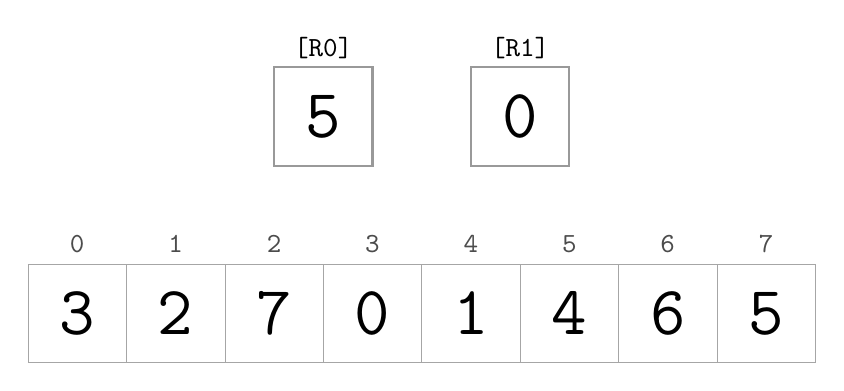
\begin{tikzpicture}
					
					\draw [gray!80,thick] (3.125,2.5) rectangle (4.375,3.75);
					\node (ACC) at (3.75,4) {\texttt{[R0]}};
					\node (ACCval) at (3.75,3.125) {\Huge{\texttt{5}}};
					
					\draw [gray!80,thick] (5.625,2.5) rectangle (6.875,3.75);
					\node (ACC) at (6.25,4) {\texttt{[R1]}};
					\node (ACCval) at (6.25,3.125) {\Huge{\texttt{0}}};
					
					\foreach [count=\i] \z in {3,2,7,0,1,4,6,5}{
						\edef\x{\number\numexpr\i-1\relax}
						\node (\x) at (\x * 1.25 + 0.625,1.5) {\textcolor{black!70}{\texttt{\x}}};
						\node (\i) at (\i * 1.25 - 0.625,0.625) {\Huge{\texttt{\z}}};	
					}
					\draw[step=1.25cm,very thin, gray!70] (0,0) grid (10,1.25);
					\end{tikzpicture}
				\end{center}
				\caption{\label{fig:3bitMemoryTape} A Simplified Memory System}
			\end{figure}
			
			We'll look at 5 different methods and how they are implemented in LMC\footnote{LMC only has one register, the accumulator. In our model R0 represents the accumulator} and ARM.
			
			\subsubsection{Immediate}
			\index{Addressing Modes!Immediate}
				The most simple form of memory addressing is immediate which is where you do not involve the memory at all. For example lets say you wanted to add 5 to what ever is in the target register. You just use a literal operand, which in most assembly languages is defined by using the \# symbol. So to complete the This requires no relation to the memory and is probably the easiest to understand. This is useful because you don't want to have to set aside memory locations or registers to store constants. Imagine how much slower your computer would run if every time it wanted to increment something it would have to look up the value of 1 in memory. 
				\begin{table}[h]
					\centering
					\begin{tabular}{l l}
						\texttt{RTL} & \RTL{[R0] = 5}\\
						\texttt{LMC} & Does not Exist. \\
						\texttt{ARM} & \mintinline{c-objdump}{MOV r0, #5}\\
					\end{tabular}
				\end{table}
				
			\subsubsection{Direct}
				Direct addressing \index{Addressing Modes!Direct}, sometimes referred to as absolute addressing is where the operand specifies the location of the data. So to use absolute addressing you would provide the location in memory or in a register. For example \mintinline{hs}{ADD R0, R0, R1} uses absolute addressing to set the contents of register 0 to be equal to register 1 plus register 0.
				
				\begin{table}[h]
					\centering
					\begin{tabular}{l l}
						\texttt{RTL} & \RTL{[R0] |$\gets$| [5]}\\
						\texttt{LMC} & \texttt{LDA 5}  \\
						\texttt{ARM} & \mintinline{c-objdump}{MOV R0, 5}\\
					\end{tabular}
				\end{table}
			
			\subsubsection{Indirect}
				In indirect addressing \index{Addressing Modes!Indirect}, the operand is specified indirectly via the contents of a pointer. For example the command \ARM{LDR R0, [R1]}, would go the memory location given by \RTL{R1} and would then take the value there and load it into \RTL{R0}. So for example, in situation below, \RTL{R1} points to \RTL{[2]}, which has a value of 7. This would then be loaded into \RTL{R0}.
				\begin{figure}[h!]
					\begin{center}
						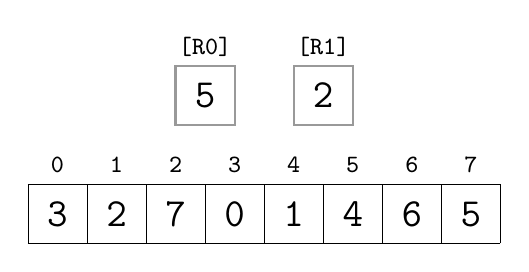
\begin{tikzpicture}
						
						\draw [gray!80,thick] (1.875,1.5) rectangle (2.625,2.25);
						\node (ACC) at (2.25,2.5) {\small{\texttt{[R0]}}};
						\node (ACCval) at (2.25,1.875) {\Large{\texttt{5}}};
						
						\draw [gray!80,thick] (3.375,1.5) rectangle (4.125,2.25);
						\node (ACC) at (3.75,2.5) {\small{\texttt{[R1]}}};
						\node (ACCval) at (3.75,1.875) {\Large{\texttt{2}}};
						
						\foreach [count=\i] \z in {3,2,7,0,1,4,6,5}{
							\edef\x{\number\numexpr\i-1\relax}
							\node (\x) at (\x * 0.75 + 0.375,1) {\small{\texttt{\x}}};
							\node (\i) at (\i * 0.75 - 0.375,0.375) {\Large{\texttt{\z}}};	
						}
						
						\draw[step=0.75cm,very thin] (0,0) grid (6,0.75);
						\end{tikzpicture}
					\end{center}
				\end{figure}
		
			\begin{table}[h]
				\centering
				\begin{tabular}{l l}
					\texttt{RTL} & \RTL{[R0] |$\gets$| [[5]]}\\
					\texttt{LMC} & \texttt{LDA 5; ADD 5XX; STA TEMP; TEMP;...; 5XX VAR 500} \footnotemark\\
					\texttt{ARM} & \ARM{MOV R1,#0; LDA R0, [R1, #5];} \\
				\end{tabular}
			\end{table}
			\footnotetext[2]{Note that for \RTL{[5] = 101} this leads to an infinite loop}
			
			\subsubsection{Register Addressing}
				Register Addressing makes use of the value of a register in order to provide more complex modes of addressing. 
				
				
			
			You most commonly find this when dealing with \ARM{BRA} instructions, 
			When you do the second instruction is now relative to last instruction. So if the next command is \texttt{ADD 4}, rather than being relating to the information in the 4\textsuperscript{th} memory location, its moves the point along 4 spaces. So instead it refers to information in the 6\textsuperscript{th} memory location. So the final result would be 20. \\
			
			If we then called \texttt{ADD -1} then we would shift the point to 1 space to the left. So it would go the fifth memory location, and then add this value.
			
			\begin{figure}[h!]
				\begin{center}
					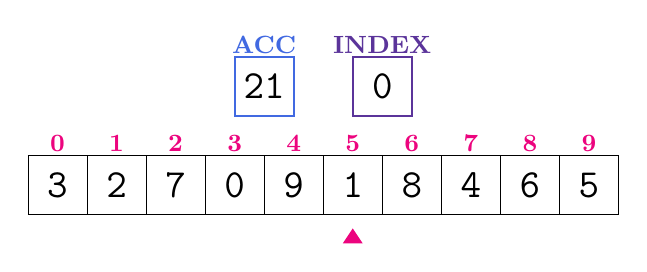
\begin{tikzpicture}
					
					\draw [RoyalBlue,thick] (2.625,1.25) rectangle (3.375,2);
					\node (ACC) at (3,2.15) {\small{\textcolor{RoyalBlue}{\textbf{ACC}}}};
					\node (ACCval) at (3,1.625) {\Large{\texttt{21}}};
					
					\draw [RoyalPurple,thick] (4.125,1.25) rectangle (4.875,2);
					\node (ACC) at (4.5,2.15) {\small{\textcolor{RoyalPurple}{\textbf{INDEX}}}};
					\node (ACCval) at (4.5,1.625) {\Large{\texttt{0}}};
					
					\foreach [count=\i] \z in {3,2,7,0,9,1,8,4,6,5}{
						\edef\x{\number\numexpr\i-1\relax}
						\node (\x) at (\x * 0.75 + 0.375,0.9) {\small{\textcolor{RubineRed}{\textbf{\x}}}};
						\node (\i) at (\i * 0.75 - 0.375,0.375) {\Large{\texttt{\z}}};	
					}
					
					\draw[fill=RubineRed!80, RubineRed, thick] (4.125,-0.2) -- +(0.1, -0.15) -- + (-0.1, -0.15) -- cycle;
					\draw[step=0.75cm,very thin] (0,0) grid (7.5,0.75);
					\end{tikzpicture}
				\end{center}
			\end{figure}
			
			\subsubsection{Indexed Addressing}
			
			Indexed addressing uses a special register called the index address. The index register is incremented each time it is referred to. The memory address given by the instruction is then addressed using the INDEX address. 
			
			\begin{figure}[h!]
				\begin{center}
					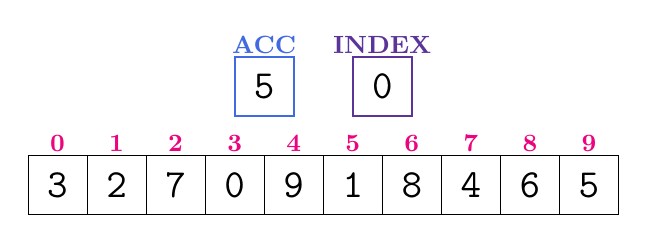
\begin{tikzpicture}
					
					\draw [RoyalBlue,thick] (2.625,1.25) rectangle (3.375,2);
					\node (ACC) at (3,2.15) {\small{\textcolor{RoyalBlue}{\textbf{ACC}}}};
					\node (ACCval) at (3,1.625) {\Large{\texttt{5}}};
					
					\draw [RoyalPurple,thick] (4.125,1.25) rectangle (4.875,2);
					\node (ACC) at (4.5,2.15) {\small{\textcolor{RoyalPurple}{\textbf{INDEX}}}};
					\node (ACCval) at (4.5,1.625) {\Large{\texttt{0}}};
					
					\foreach [count=\i] \z in {3,2,7,0,9,1,8,4,6,5}{
						\edef\x{\number\numexpr\i-1\relax}
						\node (\x) at (\x * 0.75 + 0.375,0.9) {\small{\textcolor{RubineRed}{\textbf{\x}}}};
						\node (\i) at (\i * 0.75 - 0.375,0.375) {\Large{\texttt{\z}}};	
					}
					\draw[step=0.75cm,very thin] (0,0) grid (7.5,0.75);
					\end{tikzpicture}
				\end{center}
			\end{figure}
			\index{Addressing Modes|)}
		\subsection{ARM}
		
		\subsection{Savage-1}
	
	\section{Building the Savage-1}
	
		\subsection{Clock}
			
		
		\subsection{Buses}
		
		\subsection{System Registers}
		
		\subsection{The Arithmetic Logic Unit}
		
		\subsection{Fetch, Decode Execute Cycle}
		
		\subsection{Opcodes and Operands}
		
		\subsection{The Control Unit}
		
		\subsection{I/O and Interrupts}
		
		\subsection{Pipelining}
		
	\section{Types of Processor}
		
		\subsection{Harvard and Von Neumann}
		
		\subsection{Parallel Processing}
		

		